\documentclass[a4paper,draft]{article}
\usepackage{parskip}

\def\npart {}
\def\nterm {Fall}
\def\nyear {2026}
\def\nlecturer {Anil Ada}
\def\ncourse {Undergraduate Complexity Theory}

\makeatletter
\ifx \nauthor\undefined
  \def\nauthor{Runqiu Ye}
\else
\fi

\author{Notes taken by \nauthor\vspace{5pt}\\
  Carnegie Mellon University}
\date{\nterm\ \nyear}

\usepackage{alltt}
\usepackage{amsfonts}
\usepackage{amsmath}
\usepackage{amssymb}
\usepackage{amsthm}
\usepackage{booktabs}
\usepackage{caption}
\usepackage{enumitem}
\usepackage{fancyhdr}
\usepackage{graphicx}
\usepackage{mathdots}
\usepackage{mathtools}
\usepackage{microtype}
\usepackage{multirow}
\usepackage{pdflscape}
\usepackage{pgfplots}
\usepackage{siunitx}
\usepackage{slashed}
\usepackage{tabularx}
\usepackage{tikz}
\usepackage{tkz-euclide}
\usepackage[normalem]{ulem}
\usepackage[all]{xy}
\usepackage{imakeidx}
\usepackage[includehead,includefoot,heightrounded,left=1.25in,right=1.25in]{geometry}
\usepackage{mathrsfs}
\usepackage{stmaryrd}
\usepackage{bbm}

\makeindex[intoc, title=Index]
\indexsetup{othercode={\lhead{\emph{Index}}}}

\ifx \nextra \undefined
  \usepackage[pdftex,
    hidelinks,
    pdfauthor={Dexter Chua},
    pdfsubject={\ncourse},
    pdftitle={\ncourse},
    pdfkeywords={Cambridge Mathematics Maths Math \nterm\ \nyear\ \ncourse}]{hyperref}
  \title{\ncourse}
\else
  \usepackage[pdftex,
    hidelinks,
    pdfauthor={Dexter Chua},
    pdfsubject={Cambridge Maths Notes: \ncourse\ (\nextra)},
    pdftitle={\ncourse\ (\nextra)},
    pdfkeywords={Cambridge Mathematics Maths Math \nterm\ \nyear\ \ncourse\ \nextra}]{hyperref}

  \title{\ncourse \\ {\Large \nextra}}
  \renewcommand\printindex{}
\fi

\pgfplotsset{compat=1.12}

\pagestyle{fancyplain}
\ifx \ncoursehead \undefined
  \def\ncoursehead{\ncourse}
\fi

\lhead{\emph{\nouppercase{\leftmark}}}
\ifx \nextra \undefined
  \rhead{
    \ifnum\thepage=1
    \else
      \ncoursehead
    \fi}
\else
  \rhead{
    \ifnum\thepage=1
    \else
      \ncoursehead \ (\nextra)
    \fi}
\fi
\usetikzlibrary{arrows.meta}
\usetikzlibrary{decorations.markings}
\usetikzlibrary{decorations.pathmorphing}
\usetikzlibrary{positioning}
\usetikzlibrary{fadings}
\usetikzlibrary{intersections}
\usetikzlibrary{cd}

\newcommand*{\Cdot}{{\raisebox{-0.25ex}{\scalebox{1.5}{$\cdot$}}}}
\newcommand{\pd}[2]{\frac{\partial #1}{\partial #2}}
\ifx \nhtml \undefined
\else
  \renewcommand\printindex{}
  \DisableLigatures[f]{family = *}
  \let\Contentsline\contentsline
  \renewcommand\contentsline[3]{\Contentsline{#1}{#2}{}}
  \renewcommand{\@dotsep}{10000}
  \newlength\currentparindent
  \setlength\currentparindent\parindent

  \newcommand\@minipagerestore{\setlength{\parindent}{\currentparindent}}
  \usepackage[active,tightpage,pdftex]{preview}
  \renewcommand{\PreviewBorder}{0.1cm}

  \newenvironment{stretchpage}%
  {\begin{preview}\begin{minipage}{\hsize}}%
  {\end{minipage}\end{preview}}
  \AtBeginDocument{\begin{stretchpage}}
  \AtEndDocument{\end{stretchpage}}

  \newcommand{\@@newpage}{\end{stretchpage}\begin{stretchpage}}

  \let\@real@section\section
  \renewcommand{\section}{\@@newpage\@real@section}
  \let\@real@subsection\subsection
  \renewcommand{\subsection}{\@ifstar{\@real@subsection*}{\@@newpage\@real@subsection}}
\fi
\ifx \ntrim \undefined
\else
  \usepackage{geometry}
  \geometry{
    papersize={379pt, 699pt},
    textwidth=345pt,
    textheight=596pt,
    left=17pt,
    top=54pt,
    right=17pt
  }
\fi

\ifx \nisofficial \undefined
  \let\@real@maketitle\maketitle
  \renewcommand{\maketitle}{\@real@maketitle}
\else
\fi

\newcommand{\TODO}{\textcolor{red}{\textbf{*** TO-DO ***}}}

% Theorems
\theoremstyle{definition}
\newtheorem*{aim}{Aim}
\newtheorem*{axiom}{Axiom}
\newtheorem*{claim}{Claim}
\newtheorem*{cor}{Corollary}
\newtheorem*{conjecture}{Conjecture}
\newtheorem*{defi}{Definition}
\newtheorem*{eg}{Example}
\newtheorem*{ex}{Exercise}
\newtheorem*{sol}{Solution}
\newtheorem*{fact}{Fact}
\newtheorem*{law}{Law}
\newtheorem*{lemma}{Lemma}
\newtheorem*{notation}{Notation}
\newtheorem*{prop}{Proposition}
\newtheorem*{question}{Question}
\newtheorem*{rrule}{Rule}
\newtheorem*{thm}{Theorem}
\newtheorem*{assumption}{Assumption}

\newtheorem*{remark}{Remark}
\newtheorem*{warning}{Warning}
\newtheorem*{exercise}{Exercise}

\newtheorem{nthm}{Theorem}[section]
\newtheorem{nlemma}[nthm]{Lemma}
\newtheorem{nprop}[nthm]{Proposition}
\newtheorem{ncor}[nthm]{Corollary}

\renewcommand{\labelitemi}{--}
\renewcommand{\labelitemii}{$\circ$}

\let\stdsection\section
\renewcommand\section{\newpage\stdsection}

% Strike through
\def\st{\bgroup \ULdepth=-.55ex \ULset}

%%%%%%%%%%%%%%%%%%%%%%%%%
%%%%% Maths Symbols %%%%%
%%%%%%%%%%%%%%%%%%%%%%%%%
\newcommand{\zseqinfl}[1]{\{ #1 \}_{l=0}^\infty}
\newcommand{\zseqinfj}[1]{\{ #1 \}_{j=0}^\infty}
\newcommand{\zseqinfi}[1]{\{ #1 \}_{i=0}^\infty}
\newcommand{\zseqinfn}[1]{\{ #1 \}_{n=0}^\infty}
\newcommand{\zseqinfk}[1]{\{ #1 \}_{k=0}^\infty}
\newcommand{\zseqinfm}[1]{\{ #1 \}_{m=0}^\infty}

\newcommand{\seqinfl}[1]{\{ #1 \}_{l=1}^\infty}
\newcommand{\cupinfj}{\bigcup_{j=1}^\infty}
\newcommand{\capinfj}{\bigcap_{j=1}^\infty}
\newcommand{\suminfj}{\sum_{j=1}^\infty}
\newcommand{\seqinfj}[1]{\{ #1 \}_{j=1}^\infty}
\newcommand{\cupinfi}{\bigcup_{i=1}^\infty}
\newcommand{\capinfi}{\bigcap_{i=1}^\infty}
\newcommand{\suminfi}{\sum_{i=1}^\infty}
\newcommand{\seqinfi}[1]{\{ #1 \}_{i=1}^\infty}
\newcommand{\cupinfn}{\bigcup_{n=1}^\infty}
\newcommand{\capinfn}{\bigcap_{n=1}^\infty}
\newcommand{\suminfn}{\sum_{n=1}^\infty}
\newcommand{\seqinfn}[1]{\{ #1 \}_{n=1}^\infty}
\newcommand{\cupinfk}{\bigcup_{k=1}^\infty}
\newcommand{\sqcupinfk}{\bigsqcup_{k=1}^\infty}
\newcommand{\capinfk}{\bigcap_{k=1}^\infty}
\newcommand{\suminfk}{\sum_{k=1}^\infty}
\newcommand{\seqinfk}[1]{\{ #1 \}_{k=1}^\infty}
\newcommand{\cupinfm}{\bigcup_{m=1}^\infty}
\newcommand{\capinfm}{\bigcap_{m=1}^\infty}
\newcommand{\suminfm}{\sum_{m=1}^\infty}
\newcommand{\seqinfm}[1]{\{ #1 \}_{m=1}^\infty}
\newcommand{\limsupn}{\limsup_{n \to \infty}}
\newcommand{\liminfn}{\liminf_{n \to \infty}}

\newcommand{\cupj}{\bigcup_{j=1}}
\newcommand{\capj}{\bigcap_{j=1}}
\newcommand{\sumj}{\sum_{j=1}}
\newcommand{\seqj}[1]{\{ #1 \}_{j=1}}
\newcommand{\cupi}{\bigcup_{i=1}}
\newcommand{\capi}{\bigcap_{i=1}}
\newcommand{\sumi}{\sum_{i=1}}
\newcommand{\seqi}[1]{\{ #1 \}_{i=1}}
\newcommand{\cupn}{\bigcup_{n=1}}
\newcommand{\capn}{\bigcap_{n=1}}
\newcommand{\sumn}{\sum_{n=1}}
\newcommand{\seqn}[1]{\{ #1 \}_{n=1}}
\newcommand{\cupk}{\bigcup_{k=1}}
\newcommand{\capk}{\bigcap_{k=1}}
\newcommand{\sumk}{\sum_{k=1}}
\newcommand{\seqk}[1]{\{ #1 \}_{k=1}}
\newcommand{\cupm}{\bigcup_{m=1}}
\newcommand{\capm}{\bigcap_{m=1}}
\newcommand{\summ}{\sum_{m=1}}
\newcommand{\seqm}[1]{\{ #1 \}_{m=1}}

% mathscr
\newcommand{\cscr}{\mathscr{C}}

% mathfrak 
\newcommand{\afk}{\mathfrak{A}}
\newcommand{\bfk}{\mathfrak{B}}
\newcommand{\hfk}{\mathfrak{H}}

% mathcal 
\newcommand{\acal}{\mathcal{A}}
\newcommand{\bcal}{\mathcal{B}}
\newcommand{\ccal}{\mathcal{C}}
\newcommand{\ecal}{\mathcal{E}}
\newcommand{\fcal}{\mathcal{F}}
\newcommand{\gcal}{\mathcal{G}}
\newcommand{\hcal}{\mathcal{H}}
\newcommand{\ncal}{\mathcal{N}}
\newcommand{\ocal}{\mathcal{O}}
\newcommand{\rcal}{\mathcal{R}}
\newcommand{\tcal}{\mathcal{T}}
\newcommand{\ucal}{\mathcal{U}}
\def\L{\mathcal{L}}
\def\H{\mathcal{H}}
\renewcommand{\P}{\mathcal{P}}

% mathbf
\newcommand{\dbf}{\mathbf{D}}
\newcommand{\rbf}{\mathbf{R}}

% Analysis
\newcommand{\om}{\mu^*}
\newcommand{\fs}{F_\sigma}
\newcommand{\gd}{G_\delta}
\newcommand{\mf}{\mathfrak{M}}
\newcommand{\nf}{\mathfrak{N}}
\newcommand{\Sfin}{S_{\text{fin}}}

\newcommand{\loc}{\mathrm{loc}}
\DeclareMathOperator{\leb}{Leb}
\DeclareMathOperator{\Rec}{Rec}
\DeclareMathOperator{\Cube}{Cube}
\DeclareMathOperator{\RCube}{RCube}
\newcommand{\RCuber}{\RCube_r}
\DeclareMathOperator{\Reco}{Rec^{\circ}}
\DeclareMathOperator{\Cubeo}{Cube^{\circ}}
\DeclareMathOperator{\RCubeo}{RCube^{\circ}}
\newcommand{\RCubeor}{\RCube^{\circ}_r}

% Matrix groups
\newcommand{\GL}{\mathrm{GL}}
\newcommand{\Or}{\mathrm{O}}
\newcommand{\PGL}{\mathrm{PGL}}
\newcommand{\PSL}{\mathrm{PSL}}
\newcommand{\PSO}{\mathrm{PSO}}
\newcommand{\PSU}{\mathrm{PSU}}
\newcommand{\SL}{\mathrm{SL}}
\newcommand{\SO}{\mathrm{SO}}
\newcommand{\Spin}{\mathrm{Spin}}
\newcommand{\Sp}{\mathrm{Sp}}
\newcommand{\SU}{\mathrm{SU}}
\newcommand{\U}{\mathrm{U}}
\newcommand{\Mat}{\mathrm{Mat}}

% Matrix algebras
\newcommand{\gl}{\mathfrak{gl}}
\newcommand{\ort}{\mathfrak{o}}
\newcommand{\so}{\mathfrak{so}}
\newcommand{\su}{\mathfrak{su}}
\newcommand{\uu}{\mathfrak{u}}
\renewcommand{\sl}{\mathfrak{sl}}

% Special sets
\newcommand{\C}{\mathbb{C}}
\newcommand{\CP}{\mathbb{CP}}
\newcommand{\GG}{\mathbb{G}}
\newcommand{\N}{\mathbb{N}}
\newcommand{\Q}{\mathbb{Q}}
\newcommand{\R}{\mathbb{R}}
\newcommand{\T}{\mathbb{T}}
\newcommand{\Z}{\mathbb{Z}}
% \renewcommand{\H}{\mathbb{H}}

% Brackets
\renewcommand{\bar}[1]{\overline{#1}}
\renewcommand{\tilde}[1]{\widetilde{#1}}
\renewcommand{\hat}[1]{\widehat{#1}}
\newcommand{\floor}[1]{\left\lfloor #1 \right\rfloor}
\newcommand{\ceil}[1]{\left\lceil #1 \right\rceil}
\newcommand{\abs}[1]{\left\lvert #1\right\rvert}
\newcommand{\bket}[1]{\left\lvert #1\right\rangle}
\newcommand{\brak}[1]{\left\langle #1 \right\rvert}
\newcommand{\braket}[1]{\left\langle #1 \right\rangle}
\newcommand{\bra}{\left\langle}
\newcommand{\ket}{\right\rangle}
\newcommand{\norm}[1]{\left\lVert #1\right\rVert}
\newcommand{\normalorder}[1]{\mathop{:}\nolimits\!#1\!\mathop{:}\nolimits}
\newcommand{\tv}[1]{|#1|}
\newcommand{\bbracket}[1]{\left\llbracket #1 \right\rrbracket}
\renewcommand{\vec}[1]{\boldsymbol{\mathbf{#1}}}
\DeclareMathOperator{\curl}{curl}
\DeclareMathOperator{\diverge}{div}
\DeclareMathOperator{\dist}{dist}

% not-math
\newcommand{\bolds}[1]{{\bfseries #1}}
\newcommand{\cat}[1]{\mathsf{#1}}
\newcommand{\ph}{\,\cdot\,}
\newcommand{\term}[1]{\emph{#1}\index{#1}}
\newcommand{\phantomeq}{\hphantom{{}={}}}
% Probability
\DeclareMathOperator{\ind}{\mathbf{1}}
\DeclareMathOperator{\Bernoulli}{Bernoulli}
\DeclareMathOperator{\betaD}{beta}
\DeclareMathOperator{\bias}{bias}
\DeclareMathOperator{\binomial}{binomial}
\DeclareMathOperator{\corr}{corr}
\DeclareMathOperator{\cov}{cov}
\DeclareMathOperator{\gammaD}{gamma}
\DeclareMathOperator{\mse}{mse}
\DeclareMathOperator{\multinomial}{multinomial}
\DeclareMathOperator{\Poisson}{Poisson}
\DeclareMathOperator{\Exp}{Exp}
\DeclareMathOperator{\unif}{unif}
\DeclareMathOperator{\var}{var}
\newcommand{\E}{\mathbb{E}}
\renewcommand{\Pr}{\mathbb{P}}

% Algebra
\DeclareMathOperator{\adj}{adj}
\DeclareMathOperator{\Ann}{Ann}
\DeclareMathOperator{\Aut}{Aut}
\DeclareMathOperator{\Char}{char}
\DeclareMathOperator{\disc}{disc}
\DeclareMathOperator{\dom}{dom}
\DeclareMathOperator{\fix}{fix}
\DeclareMathOperator{\Hom}{Hom}
\DeclareMathOperator{\id}{id}
\DeclareMathOperator{\image}{image}
\DeclareMathOperator{\im}{im}
\DeclareMathOperator{\tr}{tr}
\DeclareMathOperator{\Tr}{Tr}
\newcommand{\Bilin}{\mathrm{Bilin}}
\newcommand{\Frob}{\mathrm{Frob}}

% Others
\newcommand\ad{\mathrm{ad}}
\newcommand\Art{\mathrm{Art}}
\newcommand{\B}{\mathcal{B}}
\newcommand{\cU}{\mathcal{U}}
\newcommand{\Der}{\mathrm{Der}}
\newcommand{\D}{\mathrm{D}}
\newcommand{\dR}{\mathrm{dR}}
\newcommand{\exterior}{\mathchoice{{\textstyle\bigwedge}}{{\bigwedge}}{{\textstyle\wedge}}{{\scriptstyle\wedge}}}
\newcommand{\F}{\mathbb{F}}
\newcommand{\G}{\mathcal{G}}
\newcommand{\Gr}{\mathrm{Gr}}
\newcommand{\haut}{\mathrm{ht}}
\newcommand{\Hol}{\mathrm{Hol}}
\newcommand{\hol}{\mathfrak{hol}}
\newcommand{\Id}{\mathrm{Id}}
\newcommand{\lie}[1]{\mathfrak{#1}}
\newcommand{\op}{\mathrm{op}}
\newcommand{\Oc}{\mathcal{O}}
\newcommand{\pr}{\mathrm{pr}}
\newcommand{\Ps}{\mathcal{P}}
\newcommand{\pt}{\mathrm{pt}}
\newcommand{\qeq}{\mathrel{``{=}"}}
\newcommand{\Rs}{\mathcal{R}}
\newcommand{\Vect}{\mathrm{Vect}}
\newcommand{\wsto}{\stackrel{\mathrm{w}^*}{\to}}
\newcommand{\wt}{\mathrm{wt}}
\newcommand{\wto}{\stackrel{\mathrm{w}}{\to}}
% \renewcommand{\d}{\; \mathrm{d}}
\renewcommand{\d}{\, d}
\newcommand{\dd}{\partial}
\newcommand{\nsubset}{\not\subset}
\renewcommand{\epsilon}{\varepsilon}
\renewcommand{\phi}{\varphi}

\let\Im\relax
\let\Re\relax

\DeclareMathOperator{\RHS}{RHS}
\DeclareMathOperator{\LHS}{LHS}
\DeclareMathOperator{\step}{Step}
\DeclareMathOperator{\reg}{Reg}
\DeclareMathOperator{\ran}{range}
\DeclareMathOperator{\area}{area}
\DeclareMathOperator{\card}{card}
\DeclareMathOperator{\ccl}{ccl}
\DeclareMathOperator{\ch}{ch}
\DeclareMathOperator{\cl}{cl}
\DeclareMathOperator{\cls}{\overline{\mathrm{span}}}
\DeclareMathOperator{\coker}{coker}
\DeclareMathOperator{\conv}{conv}
\DeclareMathOperator{\cosec}{cosec}
\DeclareMathOperator{\cosech}{cosech}
\DeclareMathOperator{\covol}{covol}
\DeclareMathOperator{\diag}{diag}
\DeclareMathOperator{\diam}{diam}
\DeclareMathOperator{\Diff}{Diff}
\DeclareMathOperator{\End}{End}
\DeclareMathOperator{\energy}{energy}
\DeclareMathOperator{\erfc}{erfc}
\DeclareMathOperator{\erf}{erf}
\DeclareMathOperator*{\esssup}{ess\,sup}
\DeclareMathOperator{\ev}{ev}
\DeclareMathOperator{\Ext}{Ext}
\DeclareMathOperator{\fst}{fst}
\DeclareMathOperator{\Fit}{Fit}
\DeclareMathOperator{\Frac}{Frac}
\DeclareMathOperator{\Gal}{Gal}
\DeclareMathOperator{\gr}{gr}
\DeclareMathOperator{\hcf}{hcf}
\DeclareMathOperator{\Im}{Im}
\DeclareMathOperator{\Ind}{Ind}
\DeclareMathOperator{\Int}{Int}
\DeclareMathOperator{\Isom}{Isom}
\DeclareMathOperator{\lcm}{lcm}
\DeclareMathOperator{\length}{length}
\DeclareMathOperator{\Lie}{Lie}
\DeclareMathOperator{\like}{like}
\DeclareMathOperator{\Lk}{Lk}
\DeclareMathOperator{\Maps}{Maps}
\DeclareMathOperator{\orb}{orb}
\DeclareMathOperator{\ord}{ord}
\DeclareMathOperator{\otp}{otp}
\DeclareMathOperator{\poly}{poly}
\DeclareMathOperator{\rank}{rank}
\DeclareMathOperator{\rel}{rel}
\DeclareMathOperator{\Rad}{Rad}
\DeclareMathOperator{\Re}{Re}
\DeclareMathOperator*{\res}{res}
\DeclareMathOperator{\Res}{Res}
\DeclareMathOperator{\Ric}{Ric}
\DeclareMathOperator{\rk}{rk}
\DeclareMathOperator{\Rees}{Rees}
\DeclareMathOperator{\Root}{Root}
\DeclareMathOperator{\sech}{sech}
\DeclareMathOperator{\sgn}{sgn}
\DeclareMathOperator{\snd}{snd}
\DeclareMathOperator{\Spec}{Spec}
\DeclareMathOperator{\spn}{span}
\DeclareMathOperator{\stab}{stab}
\DeclareMathOperator{\St}{St}
\DeclareMathOperator{\supp}{supp}
\DeclareMathOperator{\spt}{spt}
\DeclareMathOperator{\Syl}{Syl}
\DeclareMathOperator{\Sym}{Sym}
\DeclareMathOperator{\vol}{vol}

\DeclareMathOperator{\TIME}{\mathsf{TIME}}
\DeclareMathOperator{\BPP}{\mathsf{BPP}}
\DeclareMathOperator{\BPTIME}{\mathsf{BPTIME}}
\DeclareMathOperator{\ZPP}{\mathsf{ZPP}}
\DeclareMathOperator{\RP}{\mathsf{RP}}
\DeclareMathOperator{\coRP}{\mathsf{coRP}}
\DeclareMathOperator{\PTIME}{\mathsf{P}}
\DeclareMathOperator{\NP}{\mathsf{NP}}
\DeclareMathOperator{\coNP}{\mathsf{coNP}}
\DeclareMathOperator{\EXP}{\mathsf{EXP}}

\DeclareMathOperator{\SPACE}{\mathsf{SPACE}}
\DeclareMathOperator{\NSPACE}{\mathsf{NSPACE}}
\DeclareMathOperator{\coNSPACE}{\mathsf{coNSPACE}}
\DeclareMathOperator{\LSPACE}{\mathsf{L}}
\DeclareMathOperator{\NL}{\mathsf{NL}}
\DeclareMathOperator{\coNL}{\mathsf{coNL}}
\DeclareMathOperator{\PSPACE}{\mathsf{PSPACE}}
\DeclareMathOperator{\BPL}{\mathsf{BPL}}
\DeclareMathOperator{\BQP}{\mathsf{BQP}}

\DeclareMathOperator{\SIZE}{\mathsf{SIZE}}
\DeclareMathOperator{\Ppoly}{\mathsf{P/poly}}
\DeclareMathOperator{\AC}{\mathsf{AC}}
\DeclareMathOperator{\NC}{\mathsf{NC}}
\DeclareMathOperator{\PH}{\mathsf{PH}}
\DeclareMathOperator{\size}{size}

\pgfarrowsdeclarecombine{twolatex'}{twolatex'}{latex'}{latex'}{latex'}{latex'}
\tikzset{->/.style = {decoration={markings,
          mark=at position 1 with {\arrow[scale=2]{latex'}}},
      postaction={decorate}}}
\tikzset{<-/.style = {decoration={markings,
          mark=at position 0 with {\arrowreversed[scale=2]{latex'}}},
      postaction={decorate}}}
\tikzset{<->/.style = {decoration={markings,
          mark=at position 0 with {\arrowreversed[scale=2]{latex'}},
          mark=at position 1 with {\arrow[scale=2]{latex'}}},
      postaction={decorate}}}
\tikzset{->-/.style = {decoration={markings,
          mark=at position #1 with {\arrow[scale=2]{latex'}}},
      postaction={decorate}}}
\tikzset{-<-/.style = {decoration={markings,
          mark=at position #1 with {\arrowreversed[scale=2]{latex'}}},
      postaction={decorate}}}
\tikzset{->>/.style = {decoration={markings,
          mark=at position 1 with {\arrow[scale=2]{latex'}}},
      postaction={decorate}}}
\tikzset{<<-/.style = {decoration={markings,
          mark=at position 0 with {\arrowreversed[scale=2]{twolatex'}}},
      postaction={decorate}}}
\tikzset{<<->>/.style = {decoration={markings,
          mark=at position 0 with {\arrowreversed[scale=2]{twolatex'}},
          mark=at position 1 with {\arrow[scale=2]{twolatex'}}},
      postaction={decorate}}}
\tikzset{->>-/.style = {decoration={markings,
          mark=at position #1 with {\arrow[scale=2]{twolatex'}}},
      postaction={decorate}}}
\tikzset{-<<-/.style = {decoration={markings,
          mark=at position #1 with {\arrowreversed[scale=2]{twolatex'}}},
      postaction={decorate}}}

\tikzset{circ/.style = {fill, circle, inner sep = 0, minimum size = 3}}
\tikzset{scirc/.style = {fill, circle, inner sep = 0, minimum size = 1.5}}
\tikzset{mstate/.style={circle, draw, blue, text=black, minimum width=0.7cm}}

\tikzset{eqpic/.style={baseline={([yshift=-.5ex]current bounding box.center)}}}
\tikzset{commutative diagrams/.cd,cdmap/.style={/tikz/column 1/.append style={anchor=base east},/tikz/column 2/.append style={anchor=base west},row sep=tiny}}

\definecolor{mblue}{rgb}{0.2, 0.3, 0.8}
\definecolor{morange}{rgb}{1, 0.5, 0}
\definecolor{mgreen}{rgb}{0.1, 0.4, 0.2}
\definecolor{mred}{rgb}{0.5, 0, 0}

\def\drawcirculararc(#1,#2)(#3,#4)(#5,#6){%
  \pgfmathsetmacro\cA{(#1*#1+#2*#2-#3*#3-#4*#4)/2}%
  \pgfmathsetmacro\cB{(#1*#1+#2*#2-#5*#5-#6*#6)/2}%
  \pgfmathsetmacro\cy{(\cB*(#1-#3)-\cA*(#1-#5))/%
    ((#2-#6)*(#1-#3)-(#2-#4)*(#1-#5))}%
  \pgfmathsetmacro\cx{(\cA-\cy*(#2-#4))/(#1-#3)}%
  \pgfmathsetmacro\cr{sqrt((#1-\cx)*(#1-\cx)+(#2-\cy)*(#2-\cy))}%
  \pgfmathsetmacro\cA{atan2(#2-\cy,#1-\cx)}%
  \pgfmathsetmacro\cB{atan2(#6-\cy,#5-\cx)}%
  \pgfmathparse{\cB<\cA}%
  \ifnum\pgfmathresult=1
    \pgfmathsetmacro\cB{\cB+360}%
  \fi
  \draw (#1,#2) arc (\cA:\cB:\cr);%
}
\newcommand\getCoord[3]{\newdimen{#1}\newdimen{#2}\pgfextractx{#1}{\pgfpointanchor{#3}{center}}\pgfextracty{#2}{\pgfpointanchor{#3}{center}}}

\newcommand\qedshift{\vspace{-17pt}}
\newcommand\fakeqed{\pushQED{\qed}\qedhere}

\def\Xint#1{\mathchoice
  {\XXint\displaystyle\textstyle{#1}}%
  {\XXint\textstyle\scriptstyle{#1}}%
  {\XXint\scriptstyle\scriptscriptstyle{#1}}%
  {\XXint\scriptscriptstyle\scriptscriptstyle{#1}}%
  \!\int}
\def\XXint#1#2#3{{\setbox0=\hbox{$#1{#2#3}{\int}$}
    \vcenter{\hbox{$#2#3$}}\kern-.5\wd0}}
\def\ddashint{\Xint=}
\def\dashint{\Xint-}

\newcommand\separator{{\centering\rule{2cm}{0.2pt}\vspace{2pt}\par}}

\newenvironment{own}{\color{gray!70!black}}{}

\newcommand\makecenter[1]{\raisebox{-0.5\height}{#1}}

\mathchardef\mdash="2D

\newenvironment{significant}{\begin{center}\begin{minipage}{0.9\textwidth}\centering\em}{\end{minipage}\end{center}}
\DeclareRobustCommand{\rvdots}{%
  \vbox{
    \baselineskip4\p@\lineskiplimit\z@
    \kern-\p@
    \hbox{.}\hbox{.}\hbox{.}
  }}
\DeclareRobustCommand\tph[3]{{\texorpdfstring{#1}{#2}}}
\makeatother


\begin{document}

\section{Quantum circuits}

As my final project for the Undergraduate Complexity Theory class at
Carnegie Mellon University, this is the start of a two-part blog about
quantum computation and complexity theory. The goal of this project is to
learn about the basics of quantum computation, see an example of a quantum
algorithm, and discuss the importance of quantum computation and its
connection to classical complexity theory.

In part 1, we will discuss the basics of quantum computation, quantum
circuits, and the bounded-error quantum polynomial time complexity class
$\BQP$. In part 2, we will discuss the unstructured search problem, the
quantum query model, and Grover's algorithm.

\subsection{Basics of quantum computation}

\subsubsection*{Qubits}

Bits are the basic units of classical computation, and correspondingly
\textbf{qubits} are their quantum counterparts. A classical bit can be
either be 0 or 1, but a quantum bit can be in a state of
``superposition''. When it is measured, there is some probability of
observing 0 and some probability of observing 1. We can think of this as a
coin flip represented by a vector $v = (v_1, v_2) \in \R^2$, where $v_1$
and $v_2$ are the probabilities of the 0 and 1 outcomes, respectively. For
example, the vector $(0.6, 0.4)$ gives a probability of 0.6 for observing
0 and a probability of 0.4 for observing 1.

In quantum mechanics, however, the state of a qubit is represented by a
vector $v = (v_1, v_2) \in \C^2$, where $v_i$ is called the
\textbf{amplitude} of outcome $i$. For example, in the vector $(
\frac{1}{\sqrt{2}}, \frac{i}{\sqrt{2}} )$, $\frac{1}{\sqrt{2}}$ is the
amplitude of the 0 outcome, and $\frac{i}{\sqrt{2}}$ is the amplitude of
the 1 outcome.

The measurement axiom of quantum mechanics, called the \textbf{Born rule},
says that the probability of observing a particular outcome is the squared
magnitude of its amplitude. That is, if the state is represented by $v =
(v_1, v_2) \in \C^2$, then $\abs{v_1}^2$ is the probability of observing
0, and $\abs{v_2}^2$ is the probability of observing 1. Of course, we must
have $\abs{v_1}^2 + \abs{v_2}^2 = 1$. In the example above, the
probability of observing each outcome is $\frac{1}{2}$.

We can generalize to a quantum state with $d$ outcomes, which is
represented by a complex vector $v \in \C^d$. Again, $\abs{v_i}^2$ is the
probability that a measurement produces outcome $i$. For this to be a
valid quantum state and for the probabilities to make sense, we must have
\[
  \sumi^d \abs{v_i}^2 = 1.
\]
Equivalently, $\norm{v}_2 = \sqrt{\sumi^d \abs{v_i}^2} = 1$, where
  $\norm{\cdot}_2$ is the $\ell_2$-norm on $\C^d$.

\subsubsection*{Unitary matrices}

Because the set of valid quantum states must have unit $\ell_2$-norm, the
set of viable quantum operations must preserve the $\ell_2$-norm of the
state, i.e.\ they must be isometries. An axiom of quantum mechanics
dictates that quantum operations must also be \textbf{linear}. Recall that
norm-preserving linear maps on $\C^d$ are exactly characterized by
\textbf{unitary matrices}. That is, matrices $U \in \C^{d \times d}$ such
that $U U^* = I$, where $U^*$ is the conjugate transpose of $U$.

\subsubsection*{Multi-qubit quantum computation}

After understanding single qubits, we would like to understand a quantum
system with multiple qubits, so we can build more complicated operations
and understand what it means to locally apply some quantum operation.

As a classical analogy, think of two coins $A = (0.6, 0.4)$ and $B = (0.7,
0.3)$. There are four possible states we can observe when flipping them,
namely 00, 01, 10, and 11. We can similarly use a vector in $\R^4$ to
represent their respective probabilities, namely $(0.42, 0.18, 0.28,
0.12)$.

Combining two independent quantum states works in exactly the same way,
and the machinery we use to join them is called the \textbf{tensor
product}. If we have $v \in \C^a$ and $w \in \C^b$ representing the
quantum states, the joint system is described by the tensor product $v
\otimes w \in \C^{ab}$, where $(v \otimes w)_{ij} = v_i w_j$. We can
verify that this still has unit $\ell_2$-norm. Now, we can see that if we
have an $n$-qubit state, there will be $2^n$ possible outcomes, and it is
characterized by a $2^n$-dimensional vector.

Correspondingly, for quantum operations, we have \textbf{tensor products
of matrices}. The tensor product of matrices is the unique operator which
represents the tensor product of the underlying states. That is, for
unitary $U \in \C^{a \times a}$ and $V \in \C^{b \times b}$, the tensor
product $U \otimes V$ is defined as the unique linear operator such that
\[
  (U \otimes V) (v \otimes w) = (U v) \otimes (V w)
\]
for all $v \in \C^a$ and $w \in \C^b$. The intuition is that if we apply
  a unitary to a specific qubit, it should not affect any other qubit.

\subsubsection*{Dirac notation and inner products}

To express quantum states, we use Dirac notation. The most basic
notational idea is that we will use a ``ket'', which looks like
$\bket{\cdot}$, to describe a vector that is supposed to be a quantum
state. For example, to express the 0-outcome and 1-outcome states, we have
\[
  \bket{0} = \begin{bmatrix}
    1 \\ 0
  \end{bmatrix}, \quad
  \bket{1} = \begin{bmatrix}
    0 \\ 1
  \end{bmatrix}.
\]
Now any single qubit state $\bket{\psi}$ can be written as $\bket{\psi}
  = \alpha \bket{0} + \beta \bket{1}$. To express multi-qubit states, we
  write for any $x \in \{ 0, 1 \}^n$:
\[
  \bket{x} = \bket{x_1} \otimes \dots \otimes \bket{x_n}.
\]
These are called \textbf{classical basis states}. Indeed, they form a
  basis in which to express any $n$-qubit state
\[
  \bket{\psi} = \sum_{x \in \{0, 1\}^n} \alpha_x \bket{x}.
\]

In addition to tensor products, we also have the familiar inner product.
In Dirac notation, we use a ``bra'' to express the conjugate transpose,
and the inner product of two states $\bket{\psi}, \bket{\phi} \in \C^d$ is
written as
\[
  \braket{\psi | \phi} = \sumi^d \psi_i^* \phi_i.
\]
Their outer product $\bket{\phi} \brak{\psi}$ is given by $(\bket{\phi}
  \brak{\psi})_{ij} = \phi_i \psi_j^*$. Now, an arbitrary $n$-qubit
  unitary $U$ can be characterized by
\[
  U  = \sum_{x, y \in \{0, 1\}^n} u_{x, y} \bket{x} \brak{y},
\]
where $u_{x, y} = \brak{x} U \bket{y}$. The corresponding linear-algebra
  concepts are straightforward, so we leave the proof as an exercise.

\subsubsection*{Summary — Quantum computation over $n$ qubits}

As a brief summary, for a quantum computation over $n$ qubits, the
\textbf{states} are represented as $\bket{\psi} \in \C^{2^n}$ such that
$\norm{\psi}_2^2 = \sum_{x \in \{0, 1\}^n} \abs{\braket{x | \psi}}^2= 1$.
An \textbf{operation} is a matrix $U \in \C^{2^n \times 2^n}$ with $U^* U
= U U^* = I$ (i.e.\ unitary). Applying $U$ to $\bket{\psi}$ results in the
state $U \bket{\psi}$. Finally, a \textbf{measurement} causes the state to
collapse to a specific $\bket{x}$ with probability $\abs{\braket{x |
\psi}}^2$.

\subsubsection*{Mixed state}

For the final topic of this section, we consider mixed states. The quantum
states $\bket{\psi}$ we have defined previously are called \textbf{pure
states}. We say a state is \textbf{mixed} when it represents a probability
distribution over pure states.

To see the difference between pure states and mixed states, consider the
following example. Consider the pure state $\bket{+} \coloneq
\frac{\bket{0} + \bket{1}}{\sqrt{2}}$, and consider a mixed state which is
either $\bket{0}$ or $\bket{1}$ with $50\%$ probability. Also consider the
unitary matrix $H$, which we will later see to be the \textbf{Hadamard
gate}, defined via
\[
  H = \frac{1}{\sqrt{2}} \begin{bmatrix}
    1 & 1  \\
    1 & -1
  \end{bmatrix}.
\]
Then for the pure state we have $H \bket{+} = \bket{0} $, which is
  guaranteed, but for the mixed state we have $H \bket{0} = \bket{+}=
  \frac{\bket{0} + \bket{1}}{\sqrt{2}}$ and $H \bket{1} = \bket{-} =
  \frac{\bket{0} - \bket{1}}{\sqrt{2}}$, where each happens with $50\%$
  probability. In particular, for the mixed state, the chance of measuring
  $\bket{0}$ is
\begin{align*}
  \Pr [\text{measure $\bket{0}$}]
   & = \Pr [\text{original state is $\bket{0}$}]
  \cdot \Pr [\text{measure $\bket{0}$ on $\bket{+}$}]  \\
   & \quad + \Pr [\text{original state is $\bket{1}$}]
  \cdot \Pr [\text{measure $\bket{0}$ on $\bket{-}$}]  \\
   & = \frac{1}{2} \cdot \frac{1}{2} +
  \frac{1}{2} \cdot \frac{1}{2} = \frac{1}{2}.
\end{align*}

To describe a statistical mixture of quantum states $\{ \bket{\psi_i}
\}_i$, each with probability $p_i$, we can use a \textbf{density matrix}:
\[
  \rho = \sum_i p_i \bket{\psi_i} \brak{\psi_i} \in \C^{2^n \times 2^n},
\]
where $\sum_i p_i = 1$. As it turns out, $\rho$ is a valid density
  matrix if and only if $\rho$ is a trace-$1$ positive semidefinite
  matrix.

\subsection{Computation with quantum circuits}

Recall that in classical computation, computation is performed through
Boolean circuits and gates. In quantum computation, we will use quantum
circuits with quantum gates. More concretely, an $n$-qubit quantum circuit
is a collection of unitary operations $G_1, \dots, G_m$ called gates,
applied in sequence to a subset of $n$ wires. The composition of the gates
in the circuit generates a $2^n \times 2^n$ unitary operation. We assume
that each gate is tensored with the identity operation on each wire that
it does not touch. Consider the following example with $3$ qubits and $3$
gates:

\begin{figure}[h!]
  \centering
  \includegraphics[width=0.3\textwidth]{gate_example.pdf}
\end{figure}

As shown in the figure, $G_1$ is applied to the first qubit, then $G_2$ is
applied to the second and third qubits, and finally $G_3$ is applied to
all three qubits. The unitary matrix representing this circuit is $G_3 (I
\otimes G_2) (G_1 \otimes I \otimes I)$. Notice that we can combine $G_1$
and $G_2$ into the same layer, namely $(I \otimes G_2) (G_1 \otimes I
\otimes I) = G_1 \otimes G_2$. The \textbf{depth} of a circuit is the
number of layers of gates it has, and in the above example the depth is
$2$.

Next, we introduce some common gates. The first such example is the
\textbf{controlled-NOT} or \textbf{CNOT} gate. It has the following
action:
\[
  \bket{00} \mapsto \bket{00}, \;
  \bket{01} \mapsto \bket{01}, \;
  \bket{10} \mapsto \bket{11}, \;
  \bket{11} \mapsto \bket{10}.
\]
Namely, it maps $\bket{xy}$ to $\bket{xz}$ where $z = x \oplus y$.

A related gate is the \textbf{Toffoli} gate, or controlled-controlled-NOT
gate, which maps $\bket{x} \bket{y} \bket{z} \mapsto \bket{x} \bket{y}
\bket{z \oplus xy}$. For example, we have $\bket{011} \mapsto \bket{011}$,
but $\bket{110} \mapsto \bket{111}$. Finally, we also have a \textbf{SWAP}
gate, which maps $\bket{x} \bket{y}$ to $\bket{y} \bket{x}$ for all $x, y
\in \{0, 1\}$.

Up to now, none of the gates can be used to create superposition. To
achieve superposition, the canonical choice is the \textbf{Hadamard gate},
which is defined via
\[
  H \bket{0} = \frac{\bket{0} + \bket{1}}{\sqrt{2}} \coloneq \bket{+},
  \quad
  H \bket{1} = \frac{\bket{0} - \bket{1}}{\sqrt{2}} \coloneq \bket{-}.
\]
It is worth noting that $H^2 = I$.

Notice that all of the gates we have defined so far are real. For gates
with complex entries, we first have a \textbf{phase gate} $S$ defined via
\[
  S \bket{0} = \bket{0},
  \quad
  S \bket{1} = i \bket{1}.
\]
Another type of phase gate, most commonly referred to as the $T$ gate,
  is the square root of $S$:
\[
  T \bket{0} = \bket{0},
  \quad
  T \bket{1} = e^{i \frac{\pi}{4}} \bket{1}.
\]

To see how a quantum circuit works, one way would be to explicitly compute
the unitary matrix, but it is often more helpful to instead look at how
the system evolves over a basis. This is because a linear map is fully
defined by specifying its behavior on a basis. As an exercise, try to
analyze $(H \otimes H) \operatorname{CNOT} (H \otimes H)$.

\subsection{The complexity class $\BQP$}

To define $\BQP$, we first need to discuss how a quantum circuit is
encoded. Suppose the circuit is constructed from some universal gate set,
where all the amplitudes used in the gates are efficiently computable. To
encode a quantum circuit $Q$ properly, the encoding bitstring $\bra Q
\ket$ must satisfy:
\begin{enumerate}
  \item The encoding is unique: the mapping from a circuit to its encoding
        must be injective.
  \item The encoding is not too big: if $Q$ has $m$ gates, then $\bra Q
        \ket$ has at most $\poly(m)$ bits.
  \item The encoding is not too small: if $Q$ has $m$ gates, then $\bra Q
        \ket$ has at least $m$ bits.
\end{enumerate}

With this, we say a circuit family $\seqinfn{Q_n}$ is \textbf{poly-time
uniform} if there exists a poly-time Turing machine such that on input
$1^n$, it outputs $\bra Q_n \ket$. Moreover, we define
\textbf{bounded-error quantum polynomial time ($\BQP$)} as follows: a
language $L \in \BQP$ if there is a poly-time uniform quantum circuit
family $\seqinfn{Q_n}$ and a polynomial $q$ such that for all $x \in \{0,
1\}^n$, $x \in L$ implies the probability of measuring $\bket{1}$ on the
first qubit of $Q_n (\bket{x} \otimes \bket{0^{q(n)}})$ is at least $2/3$,
and $x \notin L$ implies the probability of measuring $\bket{1}$ on the
first qubit of $Q_n (\bket{x} \otimes \bket{0^{q(n)}})$ is at most $1/3$.
Note that the $\bket{0^{q(n)}}$ states can be seen as the ``scratch
space'' for the circuit.

How does $\BQP$ compare to other classical complexity classes we know? We
begin by showing $\BPP \subset \BQP$. This can be shown by observing that
quantum circuits can directly simulate AND and NOT gates, which are
universal for classical computation. NOT is already unitary. For AND,
simply observe that applying the Toffoli gate to $\bket{x} \bket{y}
\bket{0}$ gives $\bket{x} \bket{y} \bket{x \wedge y}$. To ``fan-out'' a
particular state, we can apply CNOT to $\bket{x} \bket{0}$ to get
$\bket{x} \bket{x}$. For the random bits, we can simulate them with
$\bket{+}$. Finally, we can check that this reduction can be done
efficiently in polynomial time, so $\BPP \subset \BQP$.

For an upper bound, we have $\BQP \subset \EXP$. To prove this, note that
any $n$-qubit state can be represented as a vector in $\C^{2^n}$, and
every quantum gate on an $n$-qubit state is a unitary matrix of size $2^n
\times 2^n$. We can compute the state after applying the unitary matrix by
multiplying the matrix and the vector in $O(4^n)$ time. Simulating the
circuit requires at most polynomially many such multiplications, implying
$\BQP \subset \EXP$. This containment showcases what many think to be true
about quantum computation — to classically simulate a general quantum
computer, you need some kind of brute-force exponential-time computation.

In fact, this exponential-time algorithm is not space-efficient either. By
a theorem we will not prove here, we actually have $\BQP \subset \PSPACE$.
The idea is to assume the circuit is constructed from Toffoli and Hadamard
gates, which are computationally universal, and consider the computation
tree induced by the Hadamard gates.

\section{Grover's algorithm}

\subsection{Query complexity}

After discussing $\BQP$, we introduce another tool for comparing the power
of quantum and classical computation — \textbf{query complexity}. This can
be compared to oracle complexity in the classical setting; namely, we have
an oracle machine that tells us the answer in one step when we give an
input. In the query complexity setting, we can also learn things about a
hidden function by providing an input, and the number of times we need to
query the function to learn the property is the new measure of complexity.

For a simple example, consider some satisfiability problem characterized
by a function $f : \{0, 1\}^n \to \{0, 1\}$, and we would like to know if
there exists $x \in \{0, 1\}^n$ such that $f(x) = 1$. This is very similar
to 3SAT, and we can only query $f$ on input $x \in \{0, 1\}^n$ one at a
time. If there is at most one possible input $x$ such that $f(x) = 1$, we
have to make exponentially many queries to determine if such an $x$
exists.

To make this model more concrete, we first need to define a
\textbf{quantum oracle}. There are two useful notions, the first of which
is the \textbf{standard oracle}. The standard oracle $B_f$ acts on two
registers:
\[
  B_f \bket{x} \bket{b} = \bket{x} \bket{b \oplus f(x)}.
\]
Another useful model is the \textbf{phase oracle} $O_f$, defined via
\[
  O_f \bket{x} = (-1)^{f(x)} \bket{x}.
\]
The standard oracle $B_f$ can simulate the phase oracle $O_f$. Indeed,
\[
  B_f \bket{x} \bket{-}
  = \bket{x} \left( \frac{\bket{f(x)} - \bket{1 \oplus f(x)}}{\sqrt{2}} \right)
  = (-1)^{f(x)} \bket{x} \bket{-}
  = (O_f \bket{x}) \bket{-}.
\]
The reverse simulation is not possible from $O_f$ as defined here
  without additional access, such as controlled access to $O_f$: the phase
  oracles for $f$ and $1 - f$ differ only by an unobservable global phase,
  whereas their standard oracles are distinct.

To see a very simple example in which a quantum algorithm has an advantage
over a classical algorithm in terms of query complexity, consider the
problem of determining if a function $f : \{0, 1\} \to \{0, 1\}$ is
constant or not, i.e.\ if $f(0) = f(1)$. Classically, it is clear that we
need two queries, but we claim there is a quantum circuit for this problem
using only one query. Indeed, consider a circuit given by $H O_f H
\bket{0}$. Then we have
\begin{align*}
  \bket{0}
   & \xrightarrow{H} \frac{\bket{0} + \bket{1}}{\sqrt{2}}
  \xrightarrow{O_f} \frac{(-1)^{f(0)} \bket{0} + (-1)^{f(1)} \bket{1}}{\sqrt{2}}
  = (-1)^{f(0)} \left( \frac{\bket{0} + (-1)^{f(0) \oplus f(1)} \bket{1}}{\sqrt{2}} \right) \\
   & \xrightarrow{H} (-1)^{f(0)} \bket{f(0) \oplus f(1)}.
\end{align*}
Therefore, if $f(0) = f(1)$, we will measure $\bket{0}$ with probability
$1$, and otherwise if $f(0) \neq f(1)$, we will measure $\bket{1}$ with
probability $1$.

This phenomenon, in which a quantum algorithm has an advantage over a
classical algorithm, is called \textbf{quantum-classical separation}.

\subsection{The unstructured search problem and lower bound}

Now let us discuss a more complicated problem in which there is
quantum-classical separation — the unstructured search problem. The
unstructured search problem is defined as follows: given a function $f :
\{0, 1\}^{n} \to \{0, 1\}$ that we can query, we try to find $x \in \{0,
1\}^n$ such that $f(x) = 1$ or report that none exists.

Again, notice that this is very similar to 3SAT. In fact, all problems in
$\NP$ can be phrased as unstructured search problems. Unfortunately, in a
classical setting, exponentially many classical queries are required.
Indeed, consider the case where there is at most one input that evaluates
to $1$. Any classical deterministic algorithm may need to make all $2^n$
queries: after receiving $0$ on the first $2^n - 1$ inputs, it must still
query the final input to distinguish a marked final input from the
all-zero function. Randomness does not help — even if half of all inputs
are queried, we only have a $1/2$ chance of choosing the input that
evaluates to $1$.

Unfortunately, there is no quantum circuit that achieves polynomial query
complexity in the unstructured search problem. The following theorem by
Bennett, Bernstein, Brassard, and Vazirani gives a lower bound on the
quantum query complexity of the unstructured search problem, known as the
\textbf{BBBV lower bound}. This theorem states that the quantum query
complexity of the unstructured search problem is $\Omega (\sqrt{2^n})$. We
present the proof now.

First, notice that a generic quantum query algorithm alternates between
applying some unitary and applying some oracle. That is, after $t$
queries, the state of the system is
\[
  U_t O_f U_{t - 1} \dots U_1 O_f \bket{0^n}.
\]
A key point is that the unitaries $U_1, \dots, U_t$ are fixed and are
  independent of what the oracle does. Our goal will be to show that for
  any choice of unitaries, there is some state $\bket{y}$ that always has
  small amplitude when queried by the oracle. Because of this, it will be
  difficult for the algorithm to see if this item returns $1$, causing it
  to fail to distinguish the constant zero function and some other $f$.

First, consider the behavior on the constant zero function. Now $O_f = I$
and the algorithm should reject. After $t$ queries, the state is
\[
  \bket{\psi_t}
  \coloneq U_t U_{t - 1} \dots U_1 \bket{0^n}
  = \sum_{x \in \{0, 1\}^n} \alpha_{x, t} \bket{x}.
\]
Suppose there are $T$ total queries, and define
\[
  m_x \coloneq \sum_{t = 0}^{T - 1} \abs{\alpha_{x, t}}^2 \geq 0.
\]
Note that
\[
  \sum_{x \in \{0, 1\}^n} m_x
  = \sum_{x \in \{0, 1\}^n} \sum_{t = 0}^{T - 1} \abs{\alpha_{x, t}}^2
  = \sum_{t = 0}^{T - 1} \sum_{x \in \{0, 1\}^n}  \abs{\alpha_{x, t}}^2
  = T.
\]
Therefore, there must exist some $y \in \{0, 1\}^n$ such that $m_y \leq
  2^{-n} T$. Moreover, by Cauchy-Schwarz, we have
\[
  \sum_{t = 0}^{T - 1} \abs{\alpha_{y, t}}
  \leq \sqrt{T \sum_{t = 0}^{T - 1} \abs{\alpha_{y, t}}^2}
  = \sqrt{m_y T}
  \leq 2^{-n / 2} T.
\]
Refer to the constant zero function as the identity, and let $f$ be the
  function that is $1$ on $y$ and $0$ otherwise. Our goal is to
  distinguish the oracle for $f$ from the oracle for the identity. Let's
  consider a set of oracles $\{ O^{(t)} \}_{t = 0}^T$, where $O^{(t)}$ is
  defined to be the identity for the first $t$ queries and $f$ on the
  remaining $T - t$ queries. Now define
\[
  \bket{\phi^{(t)}}
  \coloneq U_T O^{(t)} U_{T - 1} \dots O^{(t)} U_1 \bket{0^n}
  = U_T O_f U_{T - 1} \dots O_f U_{t + 1} O_f \bket{\psi_t}.
\]
In particular, $\bket{\phi^{(T)}} = \bket{\psi_T}$ is the resulting
  state of the algorithm on the zero function, and $\bket{\phi^{(0)}}$ is
  the resulting state of the algorithm on the function $f$ we defined.
  Note that $O_f \bket{\psi_t} = \bket{\psi_t} - 2 \alpha_{y, t}
  \bket{y}$, and unitary maps are norm-preserving. It follows that for all
  $t$, we have
\begin{align*}
  \norm{\bket{\phi^{(t + 1)}} - \bket{\phi^{(t)}}}
   & = \norm{U_T O_f \dots U_{t + 2} O_f \bket{\psi_{t + 1}}
         - U_T O_f \dots U_{t + 2} O_f U_{t + 1} O_f \bket{\psi_t}}   \\
   & = \norm{(U_T O_f \dots U_{t + 2} O_f U_{t + 1}) \bket{\psi_t}
         - (U_T O_f \dots U_{t + 2} O_f U_{t + 1}) O_f \bket{\psi_t}} \\
   & = \norm{\bket{\psi_t} - O_f \bket{\psi_t}}                       \\
   & = 2 \abs{\alpha_{y, t}}.
\end{align*}

Therefore,
\[
  \norm{\bket{\phi^{(T)}} - \bket{\phi^{(0)}}}
  \leq \sum_{t = 0}^{T - 1} \norm{\bket{\phi^{(t + 1)}} - \bket{\phi^{(t)}}}
  \leq 2 \sum_{t = 0}^{T - 1} \abs{\alpha_{y, t}}
  \leq \frac{2 T}{\sqrt{2^n}}.
\]
Hence, if $T = o (\sqrt{2^n})$, then the two states are close under the
  $2$-norm, and all measurements fail to distinguish them with high
  probability. To formalize this, recall the \textbf{total variation} of
  two discrete probability distributions $p, q$:
\[
  \operatorname{TV}(p, q)
  = \frac{1}{2} \norm{p - q}_1
  = \frac{1}{2} \sum_i \abs{p_i - q_i}.
\]
Total variation determines the maximum probability with which we can
  distinguish two probability distributions. Suppose we sample from $p$
  with probability $1/2$ and sample from $q$ with probability $1/2$; the
  maximum probability with which we can infer which distribution was
  sampled is $1/2 + \operatorname{TV} (p, q) / 2$. By applying the
  following lemma, we can convert our current bound on the $2$-norm to
  $1$-norm at the cost of a constant. Therefore, we can conclude that $T =
  \Omega(2^{n / 2})$.

\textbf{Lemma.} If $\norm{\bket{\phi} - \bket{\psi}}_2 < \epsilon$, then
$\operatorname{TV} (\bket{\phi}, \bket{\psi}) \leq 2 \epsilon$.

\subsection{Grover's algorithm}

With an $\Omega(\sqrt{2^n})$ lower bound, it is natural to wonder if there
is an algorithm that runs in $O(\sqrt{2^n})$ time. The answer is yes, with
Grover's algorithm.

It turns out that Grover's algorithm depends on the number of inputs $x$
such that $f(x) = 1$. For simplicity, assume first that there is only one
marked item.

\subsubsection*{Grover diffusion operator}

We first introduce the \textbf{Grover diffusion operator}, which is
crucial for the algorithm. Its definition is
\[
  D = 2 \bket{u} \brak{u} - I,
\]
where $\bket{u} = H^{\otimes n} \bket{0^n}$ is the uniform
  superposition.

We claim that $D$ is a unitary operator that reflects about $\bket{u}$.
Moreover, $D$ can be constructed with linearly many gates in log depth. To
show $D$ is unitary, note that
\[
  D D^*
  = (2 \bket{u} \brak{u} - I) (2 \bket{u} \brak{u} - I)^*
  = 4 \bket{u} \brak{u} - 2 \bket{u} \brak{u} - 2 \bket{u} \brak{u}  + I
  = I.
\]

To see $D$ is a reflection about $\bket{u}$, consider decomposing any
state $\bket{\psi}$ orthogonally:
\[
  \bket{\psi} = \alpha \bket{u} + \beta \bket{v},
\]
where $\braket{u | v} = 0$. Then,
\[
  D \bket{\psi}
  = \alpha (2 \bket{u} \brak{u} - I) \bket{u}
  + \beta (2 \bket{u} \brak{u} - I) \bket{v}
  = \alpha \bket{u} - \beta \bket{v}.
\]

To see $D$ can be constructed with linearly many gates in log depth,
notice that $H^{\otimes n} D H^{\otimes n} = 2 \bket{0^n} \brak{0^n} - I$.
Call this $D_0$, and we just need a circuit for $D_0$. On basis states, we
have $D_0 \bket{x} = (-1)^{x_1 \vee \dots \vee x_n} \bket{x}$, so we just
need to detect if any of the qubits are $1$, which is doable with a
linear-size, log-depth circuit. Then we apply a phase gate for the answer.

\subsubsection*{Grover's algorithm}

Recall the problem statement: we want to output the marked element $s \in
\{0, 1\}^n$ such that $f(s) = 1$, or report that none exists. The
algorithm is as follows: let $\bket{\psi_0} = H^{\otimes n} \bket{0^n} =
\bket{u}$, and compute $\bket{\psi_T} = (D O_f)^T \bket{\psi_0}$. Let
$s^*$ be a measurement of $\bket{\psi_T}$, and return $s^*$ if $f(s^*) =
1$, otherwise return none. The constant $T$ that depends only on the
number of marked items (assumed to be $1$ now) will be determined later.

To understand why this works, take a geometric perspective. Our initial
state $\bket{u}$ lies in the span of $\bket{s}$ and $\bket{\Psi} =
\frac{1}{\sqrt{2^n - 1}} \sum_{x \neq s} \bket{x}$, which is the uniform
superposition of unmarked items. Indeed,
\[
  \bket{u}
  = \frac{1}{\sqrt{2^n}} \sum_x \bket{x}
  = \frac{1}{\sqrt{2^n}} \bket{s} + \frac{1}{\sqrt{2^n}} \sum_{x \neq s} \bket{x}
  = \frac{1}{\sqrt{2^n}} \bket{s} + \sqrt{1 - 2^{-n}} \bket{\Psi}.
\]
Inductively, each iteration $\bket{\psi_t} = (D O_f)^t \bket{\psi_0}$ is
  in the span of $\bket{s}$ and $\bket{\Psi}$. Indeed, we have $\alpha
  \bket{s} + \beta \bket{\Psi} \xrightarrow{O_f} - \alpha \bket{s} + \beta
  \bket{\Psi}$, and
\[
  \alpha \bket{s} + \beta \bket{\Psi}
  \xrightarrow{D} (2 \bket{u} \brak{u} - I)
  (\alpha \bket{s} + \beta \bket{\Psi})
  = 2 (\alpha \braket{u | s} + \beta \braket{u | \Psi}) \bket{u}
  - \alpha \bket{s} - \beta \bket{\Psi},
\]
where $\bket{u}$ has already been shown to be in the span, thus
  completing the proof.

Now, each iteration of $D O_f$ is a rotation in the plane spanned by
$\bket{s}$ and $\bket{\Psi}$. Note that $O_f$ reflects about $\bket{\Psi}$
and $D$ reflects about $\bket{u}$, as shown in the following figure:
\begin{figure}[h!]
  \centering
  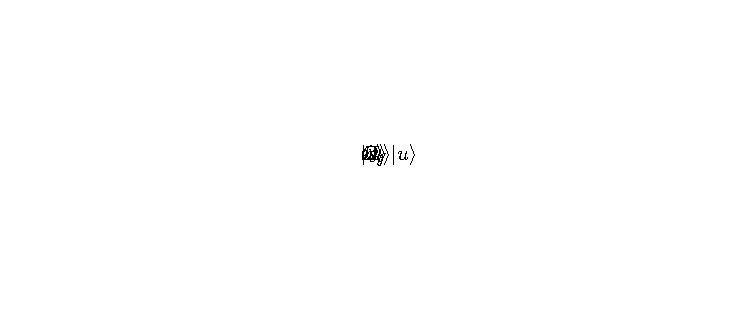
\includegraphics[width=0.9\textwidth]{grover_rotation}
\end{figure}

Hence, the evolution of the angle is given by $\theta_0, 3 \theta_0,
\dots, (2T + 1) \theta_0$. Notice that we want to reach $\pi / 2$, so we
need to choose $T \approx \pi / (4 \theta_0)$. On the other hand, we have
\[
  \theta_0 \approx \sin (\theta_0) = \braket{u | s} = 2^{- n / 2}.
\]
Hence, we choose $T = O(\sqrt{2^n})$ and the query complexity of the
  algorithm is $O(\sqrt{2^n})$. When $n$ is large enough, the final
  position $(2 T + 1) \theta_0$ is also close enough to $\pi / 2$ to
  guarantee the desired success probability.

What if there is more than one marked element? Now let $\bket{s}$ be the
uniform superposition over all $x$ such that $f(x) = 1$. If we have $m$
such elements, then the initial angle is $\braket{s | u} \approx \sqrt{m
2^{-n}}$, at least when there are not too many marked elements, so this
angle is small. In the case where there are too many elements, just
randomly sample until we find one. Then, in this case, $T = O(\sqrt{2^{n}
m^{-1}})$. Finally, what if we don't know the number of marked elements?
The trick is ``exponential search''. Namely, we consider the following
cases for $m$: $2^n, 2^{n - 1}, \dots, 4, 2, 1$. If we make all $n$
possible guesses, then we are at most a factor of $2$ off from the actual
$m$. We can check that this does not affect the correctness probability
significantly. The reverse order also gives us the $m^{-1/2}$ speedup when
there are more than $m$ marked elements.

\subsubsection*{Significance and limitations}

To conclude, we discuss some significance and limitations of Grover's
algorithm. First of all, it shows a provable quantum advantage from
$O(2^n)$ query complexity to $O(\sqrt{2^n})$ quantum query complexity. The
BBBV $\Omega (\sqrt{2^n})$ lower bound also shows that Grover's algorithm
achieves the best possible generic quantum speedup for the unstructured
search problem. The unstructured search problem also has broad
applicability. Indeed, any efficiently verifiable $f(x)$ can potentially
be searched using this algorithm, and any $\NP$ problem can be expressed
as such a problem.

However, there are some limitations. Grover's algorithm only achieves a
quadratic speedup. This is substantial but not exponential, and it does
not make $\NP$-complete problems efficient. Moreover, the complexity is
phrased in terms of query complexity, and the oracle $O_f$ may be
expensive. Therefore, it does not give a realistic speedup without the
oracle. Also, for applications like database search, there is little
advantage provided by this algorithm. It only returns one element that
satisfies the condition. Loading $N$ items already costs $O(N)$, so the
speedup is meaningless.

\end{document}
